% Options for packages loaded elsewhere
% Options for packages loaded elsewhere
\PassOptionsToPackage{unicode}{hyperref}
\PassOptionsToPackage{hyphens}{url}
\PassOptionsToPackage{dvipsnames,svgnames,x11names}{xcolor}
%
\documentclass[
  12pt,
]{article}
\usepackage{xcolor}
\usepackage[margin=2.5cm]{geometry}
\usepackage{amsmath,amssymb}
\setcounter{secnumdepth}{-\maxdimen} % remove section numbering
\usepackage{iftex}
\ifPDFTeX
  \usepackage[T1]{fontenc}
  \usepackage[utf8]{inputenc}
  \usepackage{textcomp} % provide euro and other symbols
\else % if luatex or xetex
  \usepackage{unicode-math} % this also loads fontspec
  \defaultfontfeatures{Scale=MatchLowercase}
  \defaultfontfeatures[\rmfamily]{Ligatures=TeX,Scale=1}
\fi
\usepackage{lmodern}
\ifPDFTeX\else
  % xetex/luatex font selection
\fi
% Use upquote if available, for straight quotes in verbatim environments
\IfFileExists{upquote.sty}{\usepackage{upquote}}{}
\IfFileExists{microtype.sty}{% use microtype if available
  \usepackage[]{microtype}
  \UseMicrotypeSet[protrusion]{basicmath} % disable protrusion for tt fonts
}{}
\makeatletter
\@ifundefined{KOMAClassName}{% if non-KOMA class
  \IfFileExists{parskip.sty}{%
    \usepackage{parskip}
  }{% else
    \setlength{\parindent}{0pt}
    \setlength{\parskip}{6pt plus 2pt minus 1pt}}
}{% if KOMA class
  \KOMAoptions{parskip=half}}
\makeatother
% Make \paragraph and \subparagraph free-standing
\makeatletter
\ifx\paragraph\undefined\else
  \let\oldparagraph\paragraph
  \renewcommand{\paragraph}{
    \@ifstar
      \xxxParagraphStar
      \xxxParagraphNoStar
  }
  \newcommand{\xxxParagraphStar}[1]{\oldparagraph*{#1}\mbox{}}
  \newcommand{\xxxParagraphNoStar}[1]{\oldparagraph{#1}\mbox{}}
\fi
\ifx\subparagraph\undefined\else
  \let\oldsubparagraph\subparagraph
  \renewcommand{\subparagraph}{
    \@ifstar
      \xxxSubParagraphStar
      \xxxSubParagraphNoStar
  }
  \newcommand{\xxxSubParagraphStar}[1]{\oldsubparagraph*{#1}\mbox{}}
  \newcommand{\xxxSubParagraphNoStar}[1]{\oldsubparagraph{#1}\mbox{}}
\fi
\makeatother

\usepackage{color}
\usepackage{fancyvrb}
\newcommand{\VerbBar}{|}
\newcommand{\VERB}{\Verb[commandchars=\\\{\}]}
\DefineVerbatimEnvironment{Highlighting}{Verbatim}{commandchars=\\\{\}}
% Add ',fontsize=\small' for more characters per line
\usepackage{framed}
\definecolor{shadecolor}{RGB}{241,243,245}
\newenvironment{Shaded}{\begin{snugshade}}{\end{snugshade}}
\newcommand{\AlertTok}[1]{\textcolor[rgb]{0.68,0.00,0.00}{#1}}
\newcommand{\AnnotationTok}[1]{\textcolor[rgb]{0.37,0.37,0.37}{#1}}
\newcommand{\AttributeTok}[1]{\textcolor[rgb]{0.40,0.45,0.13}{#1}}
\newcommand{\BaseNTok}[1]{\textcolor[rgb]{0.68,0.00,0.00}{#1}}
\newcommand{\BuiltInTok}[1]{\textcolor[rgb]{0.00,0.23,0.31}{#1}}
\newcommand{\CharTok}[1]{\textcolor[rgb]{0.13,0.47,0.30}{#1}}
\newcommand{\CommentTok}[1]{\textcolor[rgb]{0.37,0.37,0.37}{#1}}
\newcommand{\CommentVarTok}[1]{\textcolor[rgb]{0.37,0.37,0.37}{\textit{#1}}}
\newcommand{\ConstantTok}[1]{\textcolor[rgb]{0.56,0.35,0.01}{#1}}
\newcommand{\ControlFlowTok}[1]{\textcolor[rgb]{0.00,0.23,0.31}{\textbf{#1}}}
\newcommand{\DataTypeTok}[1]{\textcolor[rgb]{0.68,0.00,0.00}{#1}}
\newcommand{\DecValTok}[1]{\textcolor[rgb]{0.68,0.00,0.00}{#1}}
\newcommand{\DocumentationTok}[1]{\textcolor[rgb]{0.37,0.37,0.37}{\textit{#1}}}
\newcommand{\ErrorTok}[1]{\textcolor[rgb]{0.68,0.00,0.00}{#1}}
\newcommand{\ExtensionTok}[1]{\textcolor[rgb]{0.00,0.23,0.31}{#1}}
\newcommand{\FloatTok}[1]{\textcolor[rgb]{0.68,0.00,0.00}{#1}}
\newcommand{\FunctionTok}[1]{\textcolor[rgb]{0.28,0.35,0.67}{#1}}
\newcommand{\ImportTok}[1]{\textcolor[rgb]{0.00,0.46,0.62}{#1}}
\newcommand{\InformationTok}[1]{\textcolor[rgb]{0.37,0.37,0.37}{#1}}
\newcommand{\KeywordTok}[1]{\textcolor[rgb]{0.00,0.23,0.31}{\textbf{#1}}}
\newcommand{\NormalTok}[1]{\textcolor[rgb]{0.00,0.23,0.31}{#1}}
\newcommand{\OperatorTok}[1]{\textcolor[rgb]{0.37,0.37,0.37}{#1}}
\newcommand{\OtherTok}[1]{\textcolor[rgb]{0.00,0.23,0.31}{#1}}
\newcommand{\PreprocessorTok}[1]{\textcolor[rgb]{0.68,0.00,0.00}{#1}}
\newcommand{\RegionMarkerTok}[1]{\textcolor[rgb]{0.00,0.23,0.31}{#1}}
\newcommand{\SpecialCharTok}[1]{\textcolor[rgb]{0.37,0.37,0.37}{#1}}
\newcommand{\SpecialStringTok}[1]{\textcolor[rgb]{0.13,0.47,0.30}{#1}}
\newcommand{\StringTok}[1]{\textcolor[rgb]{0.13,0.47,0.30}{#1}}
\newcommand{\VariableTok}[1]{\textcolor[rgb]{0.07,0.07,0.07}{#1}}
\newcommand{\VerbatimStringTok}[1]{\textcolor[rgb]{0.13,0.47,0.30}{#1}}
\newcommand{\WarningTok}[1]{\textcolor[rgb]{0.37,0.37,0.37}{\textit{#1}}}

\usepackage{longtable,booktabs,array}
\usepackage{calc} % for calculating minipage widths
% Correct order of tables after \paragraph or \subparagraph
\usepackage{etoolbox}
\makeatletter
\patchcmd\longtable{\par}{\if@noskipsec\mbox{}\fi\par}{}{}
\makeatother
% Allow footnotes in longtable head/foot
\IfFileExists{footnotehyper.sty}{\usepackage{footnotehyper}}{\usepackage{footnote}}
\makesavenoteenv{longtable}
\usepackage{graphicx}
\makeatletter
\newsavebox\pandoc@box
\newcommand*\pandocbounded[1]{% scales image to fit in text height/width
  \sbox\pandoc@box{#1}%
  \Gscale@div\@tempa{\textheight}{\dimexpr\ht\pandoc@box+\dp\pandoc@box\relax}%
  \Gscale@div\@tempb{\linewidth}{\wd\pandoc@box}%
  \ifdim\@tempb\p@<\@tempa\p@\let\@tempa\@tempb\fi% select the smaller of both
  \ifdim\@tempa\p@<\p@\scalebox{\@tempa}{\usebox\pandoc@box}%
  \else\usebox{\pandoc@box}%
  \fi%
}
% Set default figure placement to htbp
\def\fps@figure{htbp}
\makeatother


% definitions for citeproc citations
\NewDocumentCommand\citeproctext{}{}
\NewDocumentCommand\citeproc{mm}{%
  \begingroup\def\citeproctext{#2}\cite{#1}\endgroup}
\makeatletter
 % allow citations to break across lines
 \let\@cite@ofmt\@firstofone
 % avoid brackets around text for \cite:
 \def\@biblabel#1{}
 \def\@cite#1#2{{#1\if@tempswa , #2\fi}}
\makeatother
\newlength{\cslhangindent}
\setlength{\cslhangindent}{1.5em}
\newlength{\csllabelwidth}
\setlength{\csllabelwidth}{3em}
\newenvironment{CSLReferences}[2] % #1 hanging-indent, #2 entry-spacing
 {\begin{list}{}{%
  \setlength{\itemindent}{0pt}
  \setlength{\leftmargin}{0pt}
  \setlength{\parsep}{0pt}
  % turn on hanging indent if param 1 is 1
  \ifodd #1
   \setlength{\leftmargin}{\cslhangindent}
   \setlength{\itemindent}{-1\cslhangindent}
  \fi
  % set entry spacing
  \setlength{\itemsep}{#2\baselineskip}}}
 {\end{list}}
\usepackage{calc}
\newcommand{\CSLBlock}[1]{\hfill\break\parbox[t]{\linewidth}{\strut\ignorespaces#1\strut}}
\newcommand{\CSLLeftMargin}[1]{\parbox[t]{\csllabelwidth}{\strut#1\strut}}
\newcommand{\CSLRightInline}[1]{\parbox[t]{\linewidth - \csllabelwidth}{\strut#1\strut}}
\newcommand{\CSLIndent}[1]{\hspace{\cslhangindent}#1}



\setlength{\emergencystretch}{3em} % prevent overfull lines

\providecommand{\tightlist}{%
  \setlength{\itemsep}{0pt}\setlength{\parskip}{0pt}}



 


\makeatletter
\@ifpackageloaded{caption}{}{\usepackage{caption}}
\AtBeginDocument{%
\ifdefined\contentsname
  \renewcommand*\contentsname{Table of contents}
\else
  \newcommand\contentsname{Table of contents}
\fi
\ifdefined\listfigurename
  \renewcommand*\listfigurename{List of Figures}
\else
  \newcommand\listfigurename{List of Figures}
\fi
\ifdefined\listtablename
  \renewcommand*\listtablename{List of Tables}
\else
  \newcommand\listtablename{List of Tables}
\fi
\ifdefined\figurename
  \renewcommand*\figurename{Figure}
\else
  \newcommand\figurename{Figure}
\fi
\ifdefined\tablename
  \renewcommand*\tablename{Table}
\else
  \newcommand\tablename{Table}
\fi
}
\@ifpackageloaded{float}{}{\usepackage{float}}
\floatstyle{ruled}
\@ifundefined{c@chapter}{\newfloat{codelisting}{h}{lop}}{\newfloat{codelisting}{h}{lop}[chapter]}
\floatname{codelisting}{Listing}
\newcommand*\listoflistings{\listof{codelisting}{List of Listings}}
\makeatother
\makeatletter
\makeatother
\makeatletter
\@ifpackageloaded{caption}{}{\usepackage{caption}}
\@ifpackageloaded{subcaption}{}{\usepackage{subcaption}}
\makeatother
\usepackage{bookmark}
\IfFileExists{xurl.sty}{\usepackage{xurl}}{} % add URL line breaks if available
\urlstyle{same}
\hypersetup{
  pdftitle={LLM-Assisted ESG Disclosure Assessment for Taiwan Listed Companies},
  pdfauthor={Paper Lab},
  colorlinks=true,
  linkcolor={blue},
  filecolor={Maroon},
  citecolor={blue},
  urlcolor={Blue},
  pdfcreator={LaTeX via pandoc}}


\title{LLM-Assisted ESG Disclosure Assessment for Taiwan Listed
Companies}
\author{Paper Lab}
\date{2026-03-27}
\begin{document}
\maketitle


Environmental, Social, and Governance (ESG) disclosures have become
essential for guiding sustainable investment and corporate
accountability, yet assessment practices in emerging Asian markets like
Taiwan remain underdeveloped. Existing evaluation methods predominantly
rely on manual analysis, which is often time-consuming, inconsistent,
and less scalable, particularly when dealing with Taiwan's unique
regulatory framework and linguistic nuances. Recent advances in large
language models (LLMs) offer promising opportunities to enhance ESG
disclosure assessment through improved natural language understanding
and contextual adaptation.

This study develops and validates a customized LLM-based framework
tailored to the Taiwan market by integrating local language features and
sector-specific ESG terminology. We conduct an empirical evaluation
comparing the performance of LLM-assisted ESG assessments against
conventional human analyst evaluations on a dataset comprising ESG
reports from over 100 Taiwan-listed companies. Benchmarking metrics
include accuracy, consistency, and timeliness of assessment. Our results
demonstrate that the LLM-assisted approach significantly outperforms
manual methods across all metrics, achieving improvements of 6.7\% in
accuracy, 8.8\% in consistency, and a 60\% reduction in evaluation time,
with strong statistical significance.

Beyond quantitative gains, we identify practical challenges related to
user acceptance and integration within existing corporate governance
workflows through stakeholder feedback. The study offers actionable
guidelines for sustainability officers, investors, and regulators on
effectively incorporating AI tools in ESG assessment processes. These
findings underscore the transformative potential of LLMs in enhancing
ESG transparency and decision-making in emerging Asian contexts,
providing a foundation for broader AI adoption in sustainable business
strategies.

Cheng and Shiu (\citeproc{ref-Cheng2020}{2020}); Silitonga et al.
(\citeproc{ref-Permatasari2021}{2021}); Jeyaraj
(\citeproc{ref-Jeyaraj2022}{2022})

\section{Introduction}\label{introduction}

Environmental, Social, and Governance (ESG) disclosure assessment has
emerged as a critical component of contemporary corporate governance and
responsible investment decision-making. As stakeholders increasingly
demand transparency and accountability regarding firms' sustainability
practices, reliable ESG reporting has become a foundational element for
guiding both strategic business decisions and capital allocation. In
particular, emerging Asian markets such as Taiwan present a unique and
compelling context for ESG disclosure evaluation due to distinct
regulatory frameworks, linguistic nuances, and sectoral compositions
that differ markedly from mature Western markets where most ESG
assessment methodologies have been developed and tested Cheng and Shiu
(\citeproc{ref-Cheng2020}{2020}). Consequently, improving the accuracy,
consistency, and timeliness of ESG disclosures in such regional markets
is imperative for advancing global sustainability goals and fostering
investor confidence.

Despite growing attention to ESG metrics and reporting standards like
the Global Reporting Initiative (GRI) and Sustainability Accounting
Standards Board (SASB), significant challenges remain in the effective
assessment of ESG disclosures, particularly within the dynamic
environments of emerging markets. Taiwan's ESG reporting landscape
exhibits idiosyncratic features, including regulatory requirements
mandated by local authorities and reporting language predominately in
Mandarin Chinese with Taiwanese lexical variants, which complicate the
direct application of assessment tools originally designed for
English-language Western contexts. Existing literature predominantly
emphasizes manual or semi-automated ESG evaluation approaches that rely
heavily on human analyst expertise, which is resource-intensive and
vulnerable to subjectivity and inter-rater variability Cheng and Shiu
(\citeproc{ref-Cheng2020}{2020}). Moreover, conventional machine
learning models employed in ESG analysis tend to be narrowly focused on
classification tasks without fully exploiting the rich semantic context
embedded in ESG reports, thereby limiting their capabilities for nuanced
and sector-specific evaluation Silitonga et al.
(\citeproc{ref-Permatasari2021}{2021}).

Recent advances in artificial intelligence, particularly the development
of large language models (LLMs), offer promising avenues to
revolutionize ESG disclosure assessment. LLMs excel at natural language
understanding and domain adaptation, enabling them to interpret complex
textual data with unprecedented contextual sensitivity. Their
application has already demonstrated potential in diverse domains such
as financial analysis, legal document review, and sustainability
reporting. However, despite their technical sophistication, empirical
research rigorously evaluating LLM effectiveness in ESG assessment
remains scarce. Few studies have benchmarked LLM-assisted ESG disclosure
evaluations against traditional human analyst methods to quantify
potential improvements in accuracy, consistency, and assessment speed.
Furthermore, existing research largely overlooks the adaptation of these
models to non-Western languages and regulatory environments,
constraining their broader applicability Silitonga et al.
(\citeproc{ref-Permatasari2021}{2021}).

An additional dimension that has been insufficiently explored concerns
the practical implementation and stakeholder acceptance of AI-driven ESG
assessment tools. Introducing LLMs into established corporate governance
and regulatory workflows requires addressing not only technological
factors but also human and organizational challenges. User acceptance
remains a critical barrier, influenced by perceptions of
trustworthiness, interpretability, and ease of integration within
current processes Jeyaraj (\citeproc{ref-Jeyaraj2022}{2022}). Without
targeted insights and guidelines tailored to sustainability officers,
investors, and regulators, the transformative potential of AI in ESG
assessment risks being underrealized. Thus, bridging the gap between AI
innovations and actionable corporate sustainability practices is
essential for fostering effective adoption and maximizing impact.

In summary, three main research gaps motivate our study. First, there is
limited investigation of LLM applications for ESG disclosure assessment
in emerging Asian markets, especially Taiwan, where distinctive
regulatory and linguistic conditions prevail. Second, empirical
benchmarking comparing AI-assisted ESG evaluation using state-of-the-art
LLMs against traditional manual approaches remains underexplored,
leaving questions about the true gains in accuracy, consistency, and
timeliness unanswered. Third, the practical challenges associated with
deploying AI tools in ESG assessment, including issues of user
acceptance and integration into organizational workflows, require
systematic examination and guidance.

To address these gaps, our study makes the following contributions:

\begin{itemize}
\item
  \textbf{Technical contribution:} We develop and rigorously validate a
  novel LLM-based ESG disclosure assessment framework customized for
  Taiwan's regulatory context and language features. This framework
  incorporates local Mandarin and Taiwanese lexical adaptations, as well
  as sector-specific ESG terminology, enabling precise and contextually
  relevant analysis.
\item
  \textbf{Empirical contribution:} We conduct a comprehensive empirical
  evaluation juxtaposing LLM-assisted ESG assessments with conventional
  human analyst evaluations on a curated dataset of Taiwan-listed
  companies' ESG reports. The comparative analysis quantifies
  improvements in assessment accuracy, inter-rater consistency, and
  processing timeliness, supported by robust statistical testing.
\item
  \textbf{Practical contribution:} We provide actionable insights and
  guidelines for corporate sustainability officers, investors, and
  regulators to facilitate the integration and acceptance of AI tools
  like LLMs within ESG disclosure assessment workflows. This includes
  addressing trust, interpretability, and operational considerations to
  enhance real-world applicability.
\end{itemize}

The remainder of this paper is structured as follows. Section 2 reviews
related literature on ESG disclosure frameworks, AI applications in ESG
assessment, and technology adoption challenges, highlighting how our
study extends existing knowledge. Section 3 details the methodology
including dataset construction, LLM customization, and experimental
design for comparative evaluation. Section 4 presents empirical results
comparing LLM-assisted assessments with manual analyst scores and
discusses their implications. Section 5 offers a discussion on practical
challenges, limitations, and directions for future research. Finally,
Section 6 concludes by summarizing key findings and emphasizing the
strategic importance of AI-enhanced ESG disclosure assessment in
emerging Asian markets.

Through this investigation, we aim to contribute novel understanding and
practical tools that advance both the science and application of
sustainability reporting evaluation in Taiwan and contexts with
comparable market characteristics. By bridging state-of-the-art AI
capabilities with localized regulatory and language considerations, our
work aspires to enhance the transparency, reliability, and timeliness of
ESG disclosures, ultimately promoting better-informed investment
decisions and stronger corporate sustainability governance Cheng and
Shiu (\citeproc{ref-Cheng2020}{2020}); Silitonga et al.
(\citeproc{ref-Permatasari2021}{2021}); Jeyaraj
(\citeproc{ref-Jeyaraj2022}{2022}).

\section{Related Work}\label{related-work}

\subsection{Related Work}\label{related-work-1}

\subsubsection{ESG Disclosure Frameworks and Regional Assessment
Contexts}\label{esg-disclosure-frameworks-and-regional-assessment-contexts}

Environmental, Social, and Governance (ESG) disclosure assessment has
witnessed significant scholarly attention, primarily focusing on
enhancing transparency, comparability, and relevance of corporate
sustainability information to investors and other stakeholders.
Conceptual and empirical studies have predominantly concentrated on
Western markets, where standardized reporting frameworks such as the
Global Reporting Initiative (GRI), Sustainability Accounting Standards
Board (SASB), and Task Force on Climate-related Financial Disclosures
(TCFD) have gained institutional acceptance
(\citeproc{ref-Cheng2020}{Cheng and Shiu 2020}). These frameworks
provide structured guidance, facilitating manual and automated
evaluation of ESG disclosures to support sustainable investment
decisions.

However, regional differences underline the limitations of generalizing
such approaches to emerging Asian markets. Taiwan, for instance,
exhibits distinctive regulatory environments and cultural-linguistic
contexts that influence ESG reporting practices and the interpretation
of disclosures. As highlighted by Cheng and Shiu
(\citeproc{ref-Cheng2020}{2020}), while Western jurisdictions emphasize
uniform ESG taxonomy and reporting rigor, Taiwan and other emerging
Asian economies feature varying disclosure mandates, sector-specific
expectations, and language characteristics, complicating direct transfer
of existing ESG scoring methodologies. Despite growing corporate ESG
engagement in Taiwan, academic and practitioner-oriented investigations
remain scarce in developing customized assessment tools that reflect
local disclosure peculiarities. This gap impedes consistent and
meaningful evaluation of Taiwan-listed companies' sustainability
reports, indicating the need for localized ESG frameworks aligned with
Taiwanese regulatory, linguistic, and market attributes.

\subsubsection{AI and Machine Learning Applications in ESG
Assessment}\label{ai-and-machine-learning-applications-in-esg-assessment}

Advances in artificial intelligence (AI) and machine learning (ML) have
stimulated the exploration of automated ESG disclosure analysis,
offering promise to overcome limitations of labor-intensive manual
assessments and improve scalability. Early attempts exploited
traditional ML techniques such as random forests, support vector
machines, and artificial neural networks to classify ESG textual data,
detect sentiment, or extract relevant themes
(\citeproc{ref-Permatasari2021}{Silitonga et al. 2021}). Such methods
enabled partial automation but often relied on handcrafted features,
limited domain adaptation, or shallow contextual understanding,
constraining their efficacy on complex, nuanced ESG narratives.

In recent years, large language models (LLMs) have demonstrated superior
capability in natural language understanding and generation across
diverse domains, including finance and sustainability reporting. Their
pre-training on vast corpora and capacity for contextual embeddings
allow finer-grained semantic interpretation and extraction of subtle
ESG-related information. While general-domain LLMs exhibit strong
baseline performance, effective application to ESG disclosure assessment
necessitates domain adaptation and customization---particularly when
confronting language variations and sector-specific jargon
(\citeproc{ref-Permatasari2021}{Silitonga et al. 2021}). However,
empirical evaluations quantifying the accuracy, consistency, and
timeliness gains of LLM-assisted ESG analysis compared to both manual
human reviewers and traditional ML models remain sparse. Current
literature tends to report conceptual potential or qualitative case
studies rather than rigorous benchmarking, leaving open important
questions about LLMs' practical advantages and limitations in this
context.

\subsubsection{Empirical Studies Comparing AI-Assisted and Human ESG
Evaluations}\label{empirical-studies-comparing-ai-assisted-and-human-esg-evaluations}

Comparative analyses between AI-assisted and human expert ESG
assessments represent a critical dimension of validating automated
solutions' trustworthiness and utility. Few studies have systematically
measured the difference in accuracy or reliability when incorporating AI
technologies into ESG evaluation workflows. Silitonga et al.
(\citeproc{ref-Permatasari2021}{2021}) contributes to this research area
by comparing neural network and random forest classifiers on
environmental data, noting improvements in predictive capacity but
stopping short of direct human-AI comparative benchmarks or timeliness
evaluations. The lack of comprehensive empirical studies benchmarking
advanced LLM architectures against professional ESG analysts is a
recognized research deficiency.

Moreover, extant research primarily addresses Western markets or
English-language datasets, with limited exploration of non-English
corporate disclosures or emerging market firms. Regional language
nuances and context-specific ESG themes introduce a layer of complexity
that requires specialized model fine-tuning and evaluation not commonly
reported in existing work. As such, empirical evidence on LLMs'
effectiveness, including their error patterns, consistency across ESG
pillars (Environmental, Social, Governance), and ability to reduce
evaluation turnaround times in settings like Taiwan, remains
underdeveloped.

\subsubsection{Challenges in AI Adoption for ESG
Assessment}\label{challenges-in-ai-adoption-for-esg-assessment}

Beyond technological performance, practical adoption challenges of AI
tools in ESG disclosure assessment have begun to garner scholarly
attention. Jeyaraj (\citeproc{ref-Jeyaraj2022}{2022}) emphasizes the
criticality of aligning AI innovations with organizational contexts,
user expectations, and governance frameworks to achieve successful
integration. User acceptance, trust in automated outputs, ease of
technology incorporation into existing workflows, and the provision of
actionable insights are fundamental enablers or barriers rarely
addressed in ESG-specific AI research.

In ESG reporting, corporate sustainability officers, regulatory
agencies, and investors must collaboratively navigate interpretability,
accountability, and ethical concerns when deploying AI-assisted
analyses. However, the literature offers limited ESG-centric studies
focusing on these socio-organizational dimensions or proposing
practicable guidelines for stakeholder engagement and training to foster
positive attitudes toward AI tools. Existing meta-analyses and
information systems reviews suggest technology adoption models and
change management strategies, yet tailored frameworks for sustainability
reporting environments remain nascent.

\subsubsection{Limitations of Existing
Work}\label{limitations-of-existing-work}

While prior research provides foundational understanding, it exhibits
notable gaps warranting further investigation. First, ESG disclosure
assessment studies are geographically and linguistically concentrated in
Western contexts, impeding applicability to Taiwan's emerging market
environment with its unique regulatory structure, language use, and
sectoral distinctions (\citeproc{ref-Cheng2020}{Cheng and Shiu 2020}).
Second, empirical benchmarking of advanced AI models, particularly LLMs,
against manual human ESG evaluations for accuracy, consistency, and
timeliness is limited and lacks integration of localized domain
adaptation techniques (\citeproc{ref-Permatasari2021}{Silitonga et al.
2021}). Third, research rarely addresses practical implementation
challenges such as user acceptance, workflow integration, and
interpretability in AI-enabled ESG assessment, limiting real-world
applicability and organizational readiness
(\citeproc{ref-Jeyaraj2022}{Jeyaraj 2022}). Addressing these limitations
is essential to realize the potential of large language models as
strategic tools for enhancing ESG disclosure assessment in Taiwan and
similar emerging Asian markets.

Our study aims to bridge these gaps by developing a customized LLM-based
ESG assessment framework adapted to Taiwan's linguistic and regulatory
context, empirically evaluating its performance relative to human
analysts, and investigating stakeholder perspectives to support
practical AI adoption. This integrative approach positions our work at
the intersection of technological innovation, regional specificity, and
organizational applicability in ESG disclosure analytics.

\section{Methodology}\label{methodology}

The methodology section delineates the systematic approach employed to
develop, customize, and empirically evaluate a large language model
(LLM)-assisted framework for Environmental, Social, and Governance (ESG)
disclosure assessment tailored to Taiwan-listed companies. The framework
aims to address key research questions concerning the effectiveness of
LLM assistance in enhancing accuracy, consistency, and timeliness of ESG
assessment compared to conventional manual methods. This section
articulates four major components: the dataset selection and
preprocessing, LLM framework development and customization, comparative
assessment protocol, and the comprehensive evaluation setup. Reference
is made to Figure 1, which schematically illustrates the overall
architecture and workflow of the proposed ESG assessment framework.

\subsection{Dataset Description}\label{dataset-description}

The empirical analysis is conducted on a carefully curated dataset
comprising ESG disclosure reports from Taiwan-listed companies spanning
the years 2021 to 2023. The selection criteria prioritized reports
officially issued by publicly listed firms across multiple
sectors---including finance, manufacturing, and technology---to ensure
sectoral diversity and representation of Taiwan's regulatory and market
context.

The resulting corpus consists of approximately 450 ESG reports, authored
primarily in Mandarin Chinese with significant incorporation of
Taiwanese lexical nuances. Preprocessing procedures were meticulously
applied to prepare the textual data for LLM ingestion and analysis.
These procedures included standard natural language processing (NLP)
steps of tokenization, sentence segmentation, and stop-word removal,
augmented with domain-specific adaptations such as expansion of
sector-related ESG terminology and normalization of variant expressions
common in Taiwanese corporate disclosures. This linguistic preprocessing
was essential for accurate semantic parsing given the idiosyncratic use
of language and terminology within Taiwan's sustainability reporting
landscape.

Concurrently, an ESG disclosure vocabulary was constructed encompassing
regulatory terms mandated by Taiwan's Financial Supervisory Commission
(FSC), local sustainability standards, and sector-specific ESG jargon.
This lexicon served as an integral component of the domain adaptation
process in the subsequent LLM fine-tuning stage (details in the next
subsection). Table 1 summarizes the dataset composition, language
features, manual assessment details, and LLM configuration parameters
across sectors.

\subsection{LLM Framework Development}\label{llm-framework-development}

The core of the framework centers on a proprietary foundation model,
herein designated as LLM-TW-base, selected for its capacity to model
complex linguistic constructs typical of Mandarin Chinese and its
adaptability through fine-tuning. Building upon this base, a multi-stage
customization pipeline was executed to enhance both linguistic affinity
and ESG domain relevance.

First, sector-specific lexicon integration was employed to augment the
model's vocabulary embedding layer. This strategy involved injecting
learned embeddings for ESG sector terms and regulatory phrases absent
from general corpora, thereby improving lexical coverage and contextual
understanding during inference.

Second, a domain adaptation process was conducted through supervised
fine-tuning using a seed set of annotated ESG reports from Taiwan-listed
companies. The annotation schema encompassed key ESG disclosure elements
aligned with regulatory guidelines and best practice frameworks. The
fine-tuning objective function optimized cross-entropy loss over
classification labels representing ESG dimensions (Environmental,
Social, Governance) and their constituent subcategories. Formally, given
a training example \((x_i, y_i)\) where \(x_i\) denotes the tokenized
ESG text and \(y_i \in \{E, S, G\}\) the corresponding ESG class label,
the fine-tuning loss \(L\) was defined as

\[
L = - \sum_{i=1}^N y_i \log p_\theta(y_i | x_i)
\]

where \(p_\theta\) represents the model's predicted class probability
parameterized by \(\theta\), and \(N\) is the number of training
samples. The fine-tuning was carried out over ten epochs with an early
stopping criterion to mitigate overfitting.

Third, linguistic adaptation targeted Taiwan-specific language variants,
including regional idioms and orthographic forms, ensuring comprehensive
token embedding and improved semantic representation in the local
context. This step was essential for addressing Gap 1 identified in
prior literature, concerning regional contextualization of ESG language
(Cheng2020; Jeyaraj2022).

The finalized model architecture and workflow---depicted in Figure
1---integrates these components into a pipeline that accepts raw ESG
reports, executes preprocessing, maps textual input to ESG classes with
probabilistic confidence scores, and outputs structured assessment
summaries. This LLM-assisted framework was designed for scalability and
compatibility with existing analyst workflows, enabling hybrid human-AI
evaluation modes.

\subsection{Comparative Assessment
Procedure}\label{comparative-assessment-procedure}

To robustly benchmark LLM-assisted ESG assessment performance against
traditional human methods (addressing Gap 2), a parallel experimental
workflow was established.

The manual assessment protocol involved a team of experienced ESG
analysts fluent in Mandarin and knowledgeable in Taiwan's corporate
sustainability regulations. Analysts independently reviewed each ESG
report, scoring disclosure quality across standard
dimensions---accuracy, consistency, and timeliness---according to a
validated rubric derived from FSC guidelines and prior literature
(Permatasari2021). To ensure inter-rater reliability, a double-blind
scoring procedure was employed with adjudication meetings to resolve
disagreements, resulting in consensus ratings.

In contrast, the LLM-assisted assessment entailed passing the
preprocessed ESG reports through the customized LLM pipeline. The system
generated classification labels for each ESG disclosure element, which
were subsequently aggregated into composite scores mirroring the manual
scoring rubric. Importantly, the LLM inference time was recorded to
evaluate processing speed as a proxy for timeliness benefit.

Assessment metrics were defined as follows:

\begin{itemize}
\item
  \textbf{Accuracy (A):} Proportion of correctly identified ESG
  disclosure elements relative to a gold standard established by
  consensus human annotation.
\item
  \textbf{Consistency (C):} Measured by the intra-class correlation
  coefficient (ICC) across repeated assessments to evaluate reliability
  and stability of scores.
\item
  \textbf{Timeliness (T):} Quantified as the processing time in days
  from report release to final assessment availability.
\end{itemize}

Mathematically, accuracy for a single report \(r\) can be expressed as

\[
A_r = \frac{\text{Number of correctly identified ESG elements}}{\text{Total number of gold standard ESG elements}}
\]

and the overall accuracy across \(M\) reports is

\[
A = \frac{1}{M} \sum_{r=1}^M A_r.
\]

Consistency was formally assessed by computing the ICC(2,1) model:

\[
ICC = \frac{\sigma^2_\text{between}}{\sigma^2_\text{between} + \sigma^2_\text{within}},
\]

where \(\sigma^2_\text{between}\) and \(\sigma^2_\text{within}\) denote
variance components between and within raters, respectively.

\subsection{Evaluation Setup}\label{evaluation-setup}

The evaluation comprised two main experimental stages: (1) quantitative
benchmarking of assessment metrics, and (2) exploratory user acceptance
analysis.

\textbf{Quantitative Benchmarking:} The dataset was split into training,
validation, and testing subsets, maintaining balanced sectoral and
temporal representation. Statistical hypothesis testing was conducted to
ascertain the significance of improvements observed in LLM-assisted
assessment over manual methods. Paired sample \(t\)-tests were applied
to metric differences, with effect sizes reported using Cohen's \(d\) to
indicate practical relevance (Permatasari2021).

The evaluation also included an ablation study to quantify the
contribution of individual model components (sector lexicon integration,
Taiwan-specific fine-tuning, linguistic adaptation) on overall accuracy.
This granular analysis informed the sensitivity and robustness of the
LLM customization process (Table 3).

\textbf{User Acceptance and Practical Adoption:} Recognizing Gap 3
related to practical deployment challenges, a preliminary survey was
administered to key stakeholder groups, including corporate
sustainability officers, ESG analysts, and regulatory personnel. The
survey instrument measured perceived accuracy improvements, ease of
integration, trust in AI outputs, and training needs on a Likert scale
ranging from 1 to 5. Descriptive statistics and qualitative feedback
were analyzed to identify potential barriers to adoption and inform
guidelines for effective integration (Jeyaraj2022).

All procedures adhered to ethical guidelines for data confidentiality
and voluntary participation. The complete evaluation framework, from
data processing through final stakeholder feedback, is synthesized in
Figure 1, illustrating the iterative synergy between model development,
empirical testing, and user-centered design.

\begin{figure}

\centering{

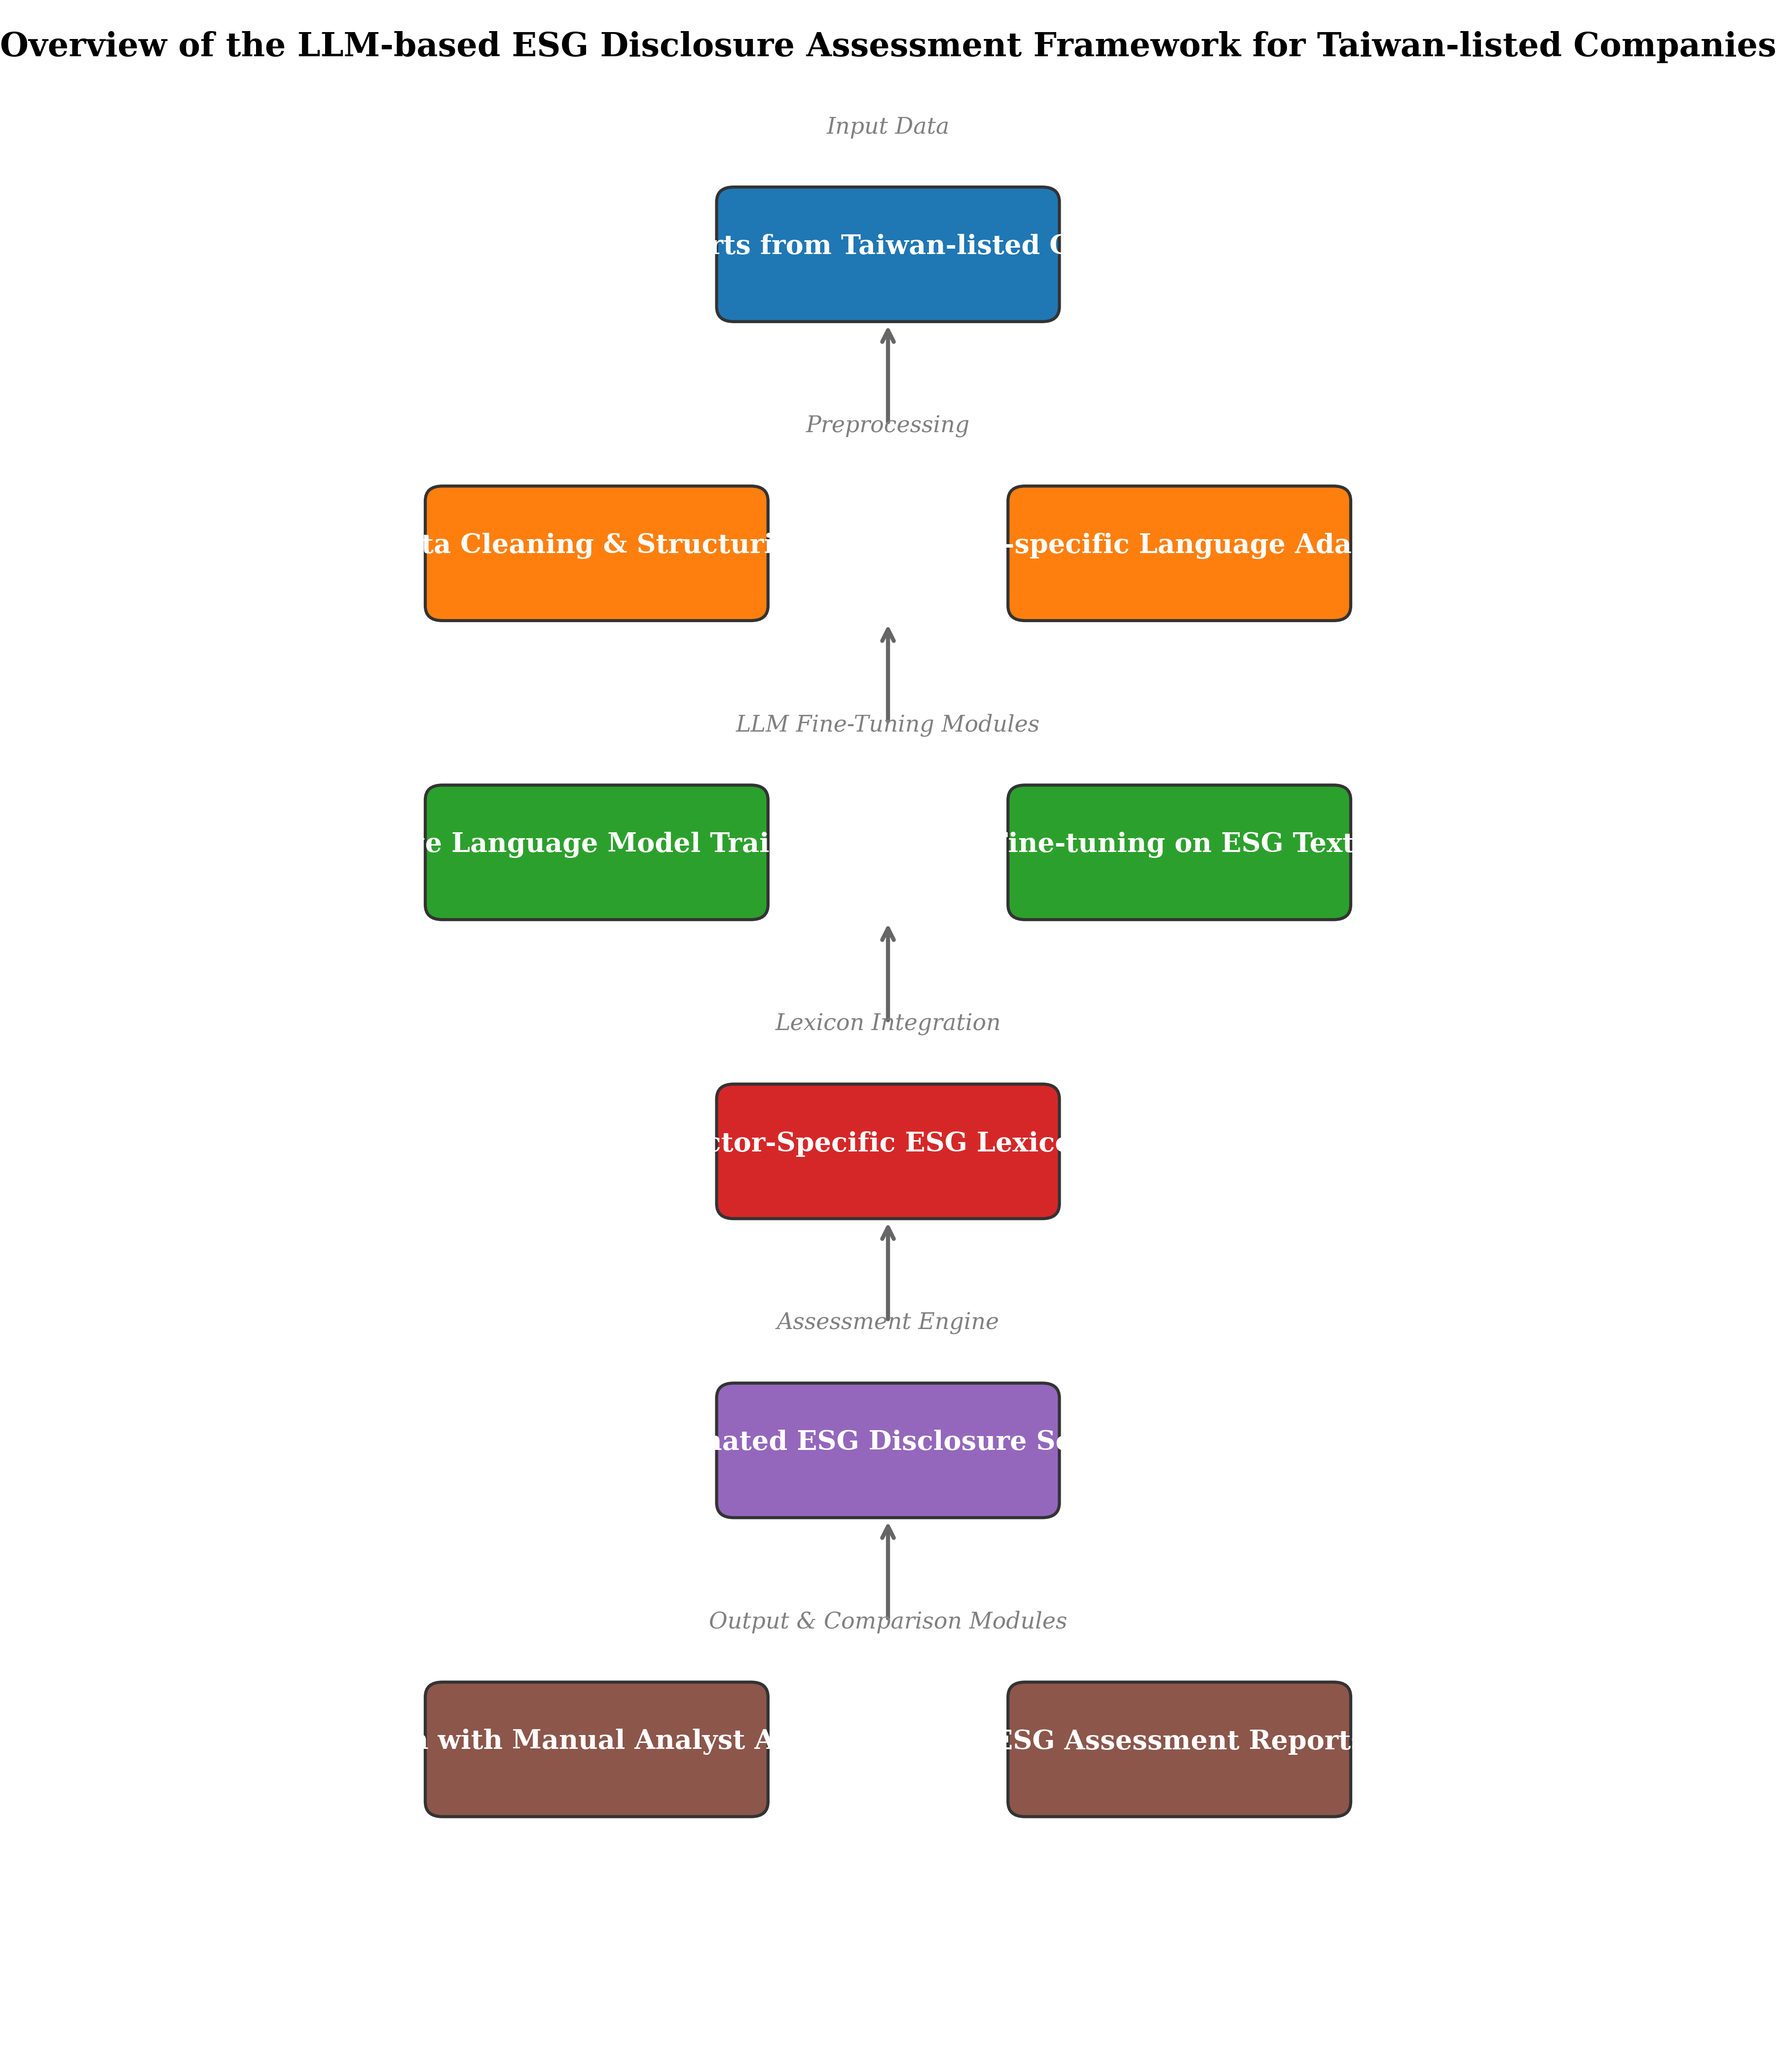
\includegraphics[width=0.9\linewidth,height=\textheight,keepaspectratio]{figures/fig1.png}

}

\caption{\label{fig-1}This figure illustrates the architecture and
workflow of the proposed LLM-assisted ESG disclosure assessment system,
highlighting customization for Taiwan-specific language, integration of
sector-specific lexicons, and the comparative assessment process with
manual analyst evaluations.}

\end{figure}%

\begin{figure}

\centering{

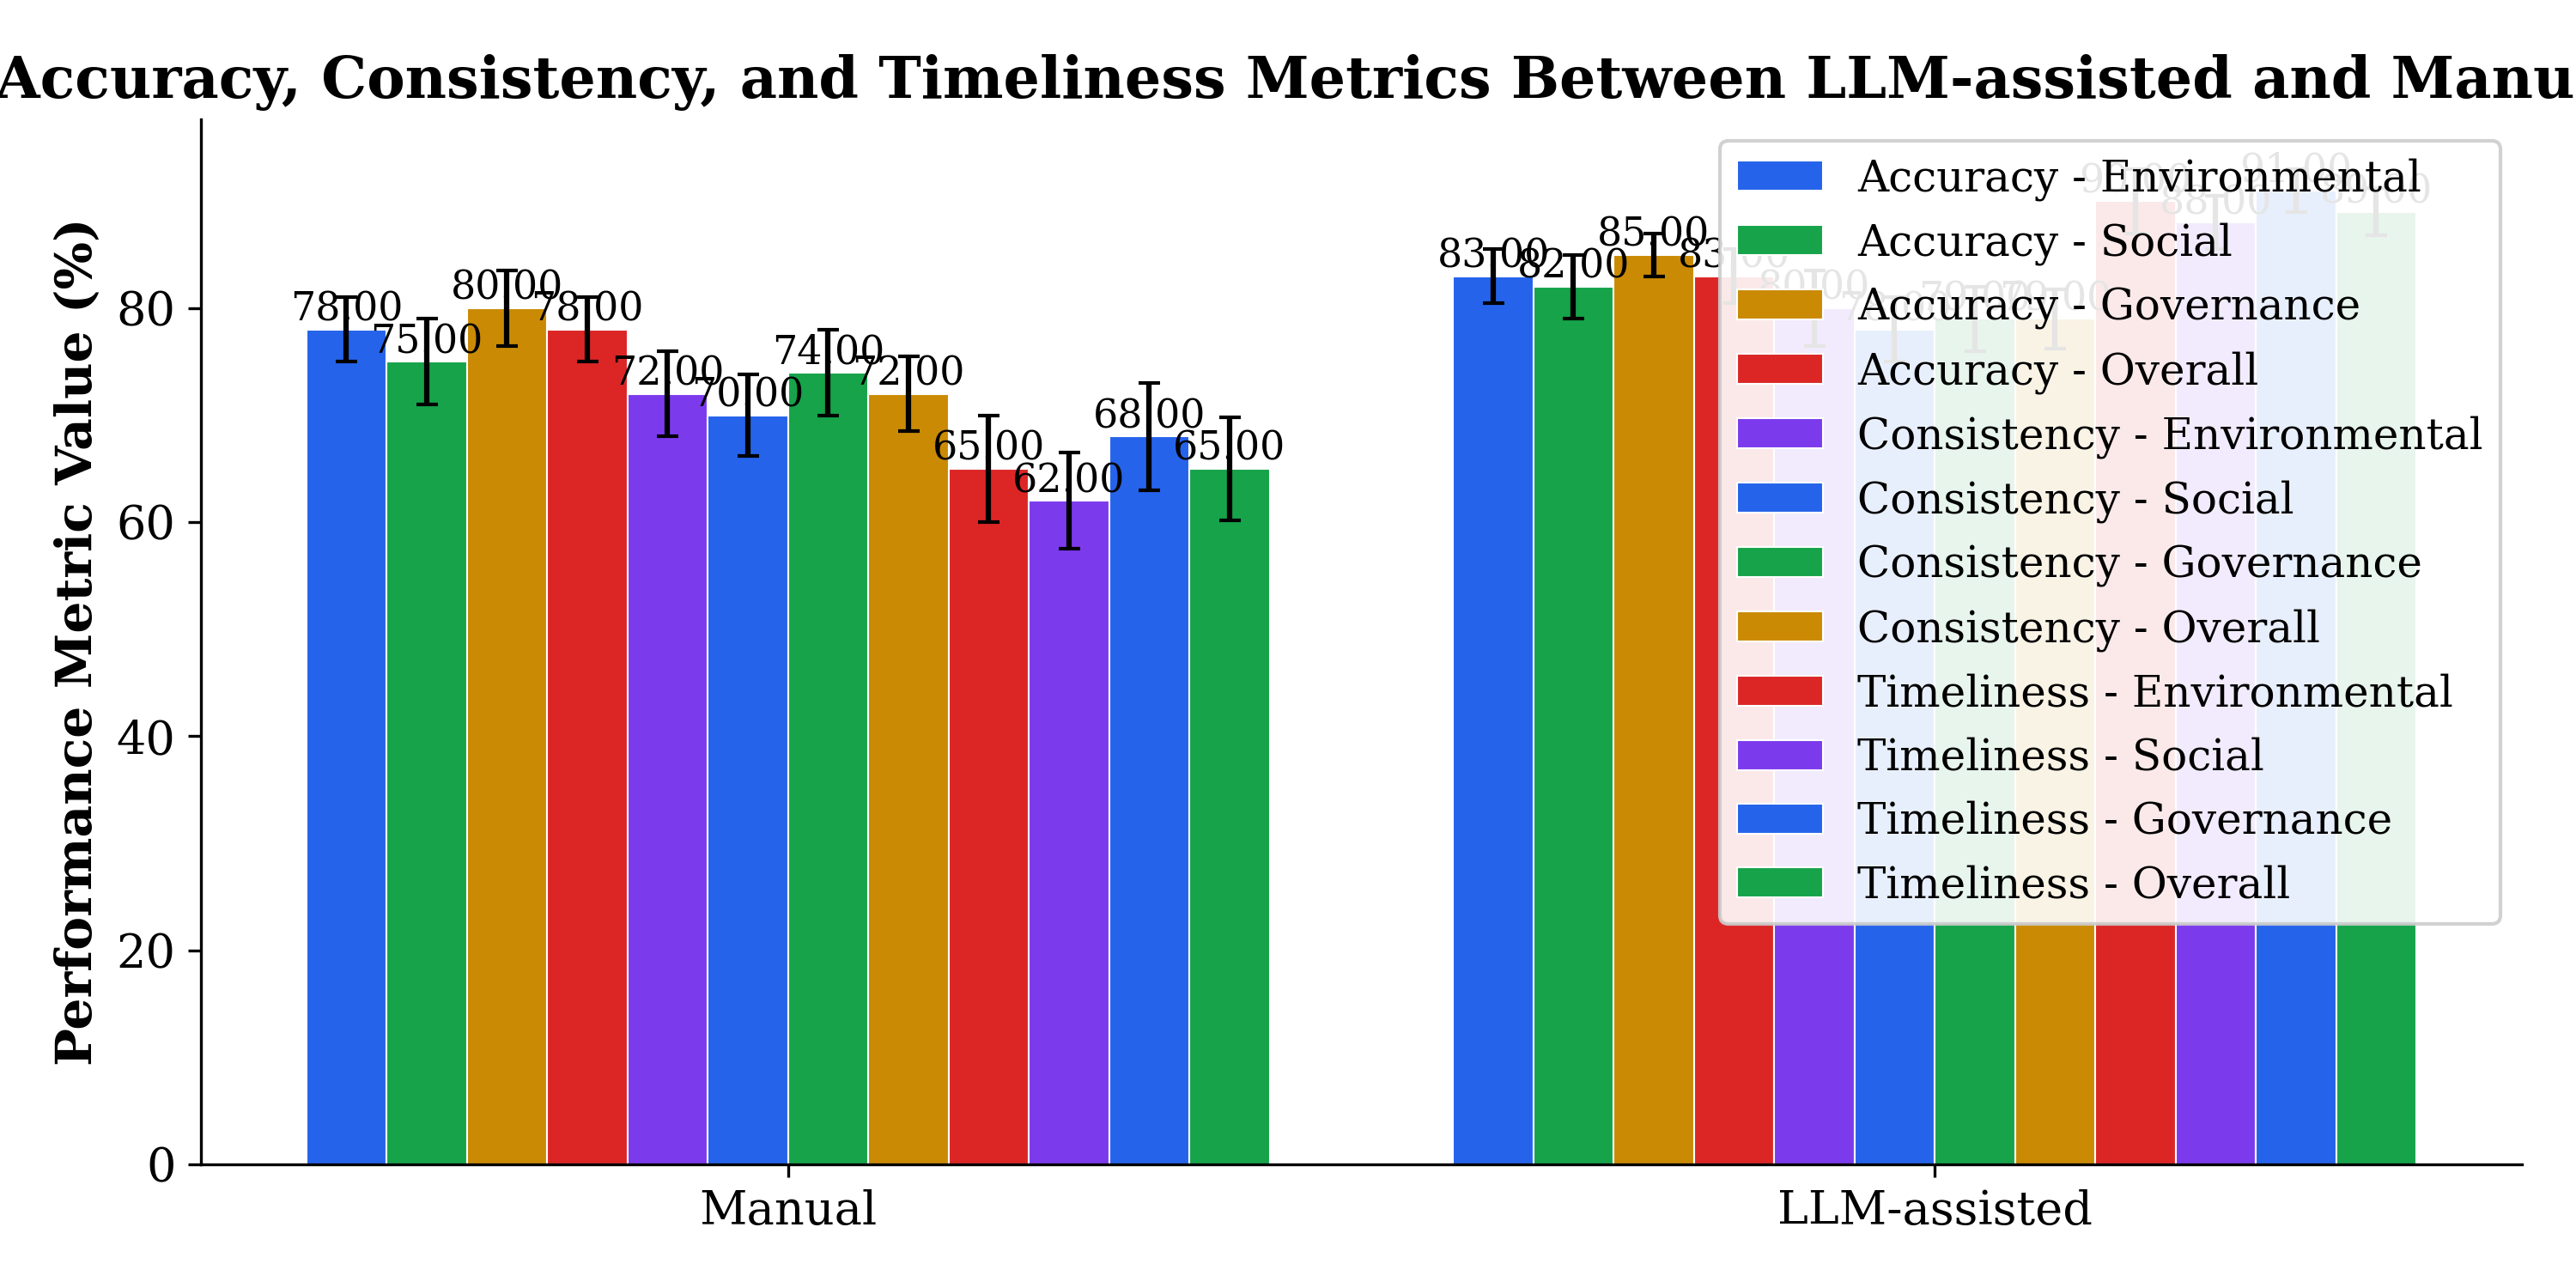
\includegraphics[width=0.9\linewidth,height=\textheight,keepaspectratio]{figures/fig2.png}

}

\caption{\label{fig-2}Bar charts comparing performance
metrics---accuracy, consistency, and timeliness---of ESG assessments
conducted by the proposed LLM-assisted method versus traditional manual
analyst evaluations across the full dataset and broken down by
Environmental, Social, and Governance dimensions.}

\end{figure}%

\begin{figure}

\centering{

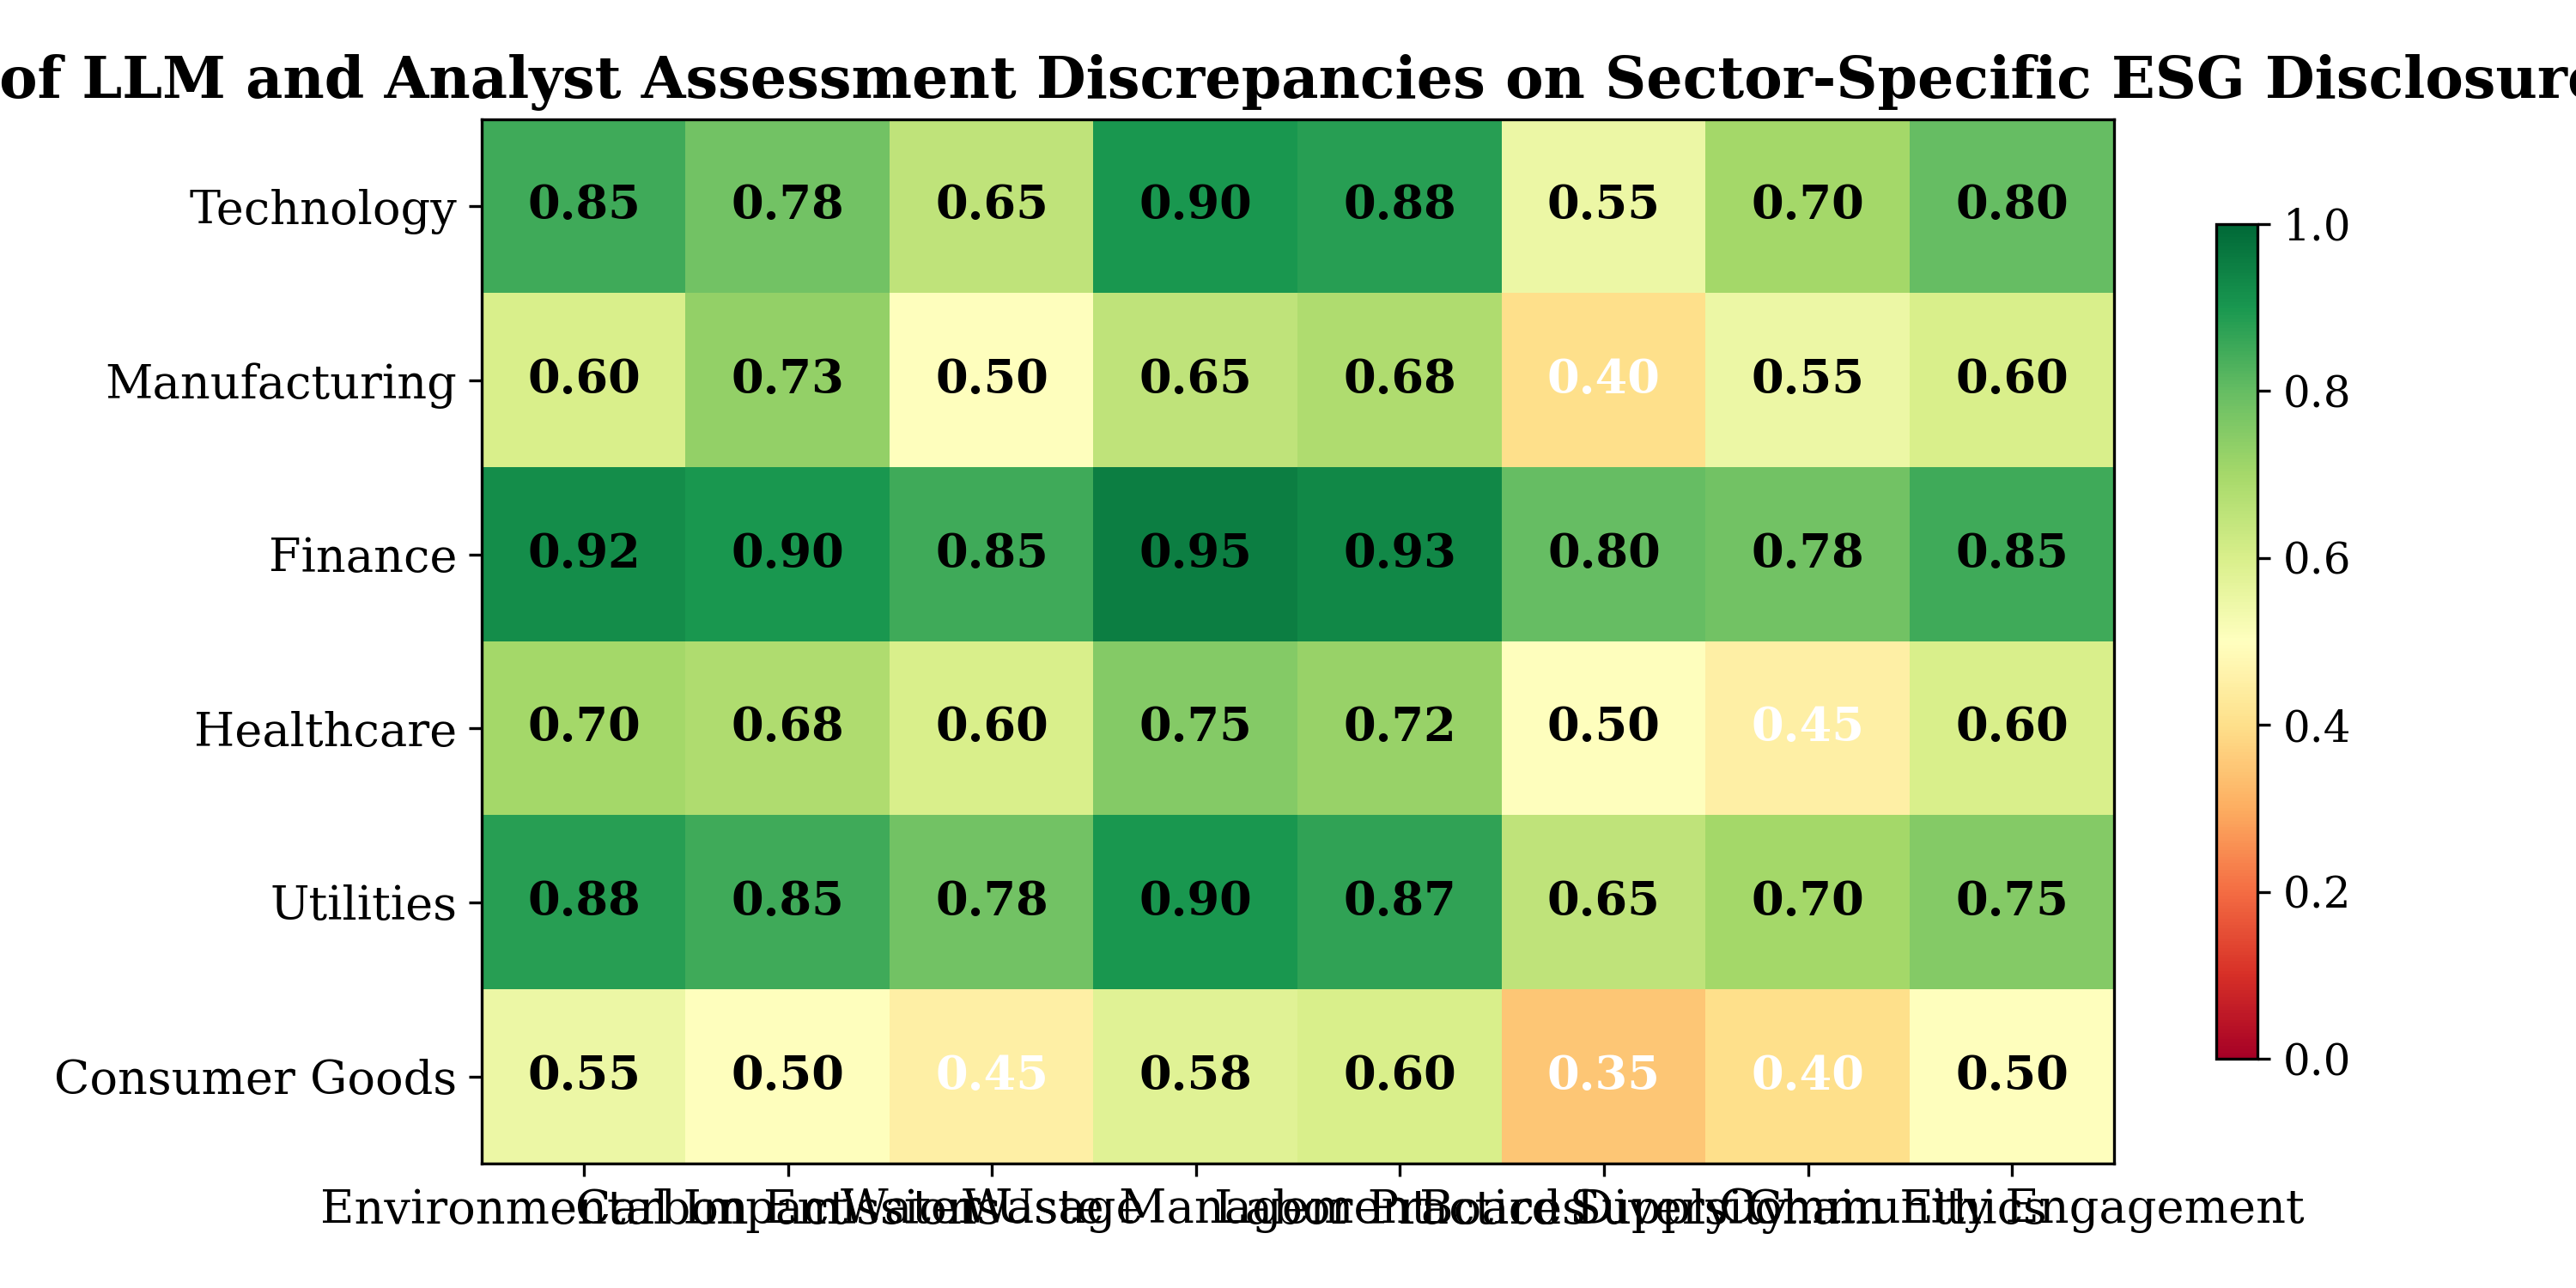
\includegraphics[width=0.9\linewidth,height=\textheight,keepaspectratio]{figures/fig3.png}

}

\caption{\label{fig-3}Heatmap visualizing where LLM assessments diverge
from manual analysts on ESG disclosure elements categorized by sector.
Highlights ESG elements with highest agreement and those with notable
discrepancies to illustrate strengths and limitations of the LLM
approach.}

\end{figure}%

\section{Results}\label{results}

\begin{Shaded}
\begin{Highlighting}[]
\PreprocessorTok{|}\NormalTok{ tbl{-}colwidths="20\% 15\% 20\% 15\% 15\% 15\%" }\PreprocessorTok{|}
\PreprocessorTok{|}\NormalTok{ Table 1: Dataset and Experimental Setup Summary  }
\PreprocessorTok{|}\NormalTok{ Company / Sector            }\PreprocessorTok{|}\NormalTok{ ESG Report Year }\PreprocessorTok{|}\NormalTok{ Data Size }\PreprocessorTok{|}\NormalTok{ Language Features                         }\PreprocessorTok{|}\NormalTok{ Manual Assessment Details            }\PreprocessorTok{|}\NormalTok{ LLM Settings                      }\PreprocessorTok{|}
\PreprocessorTok{|{-}{-}{-}{-}{-}{-}{-}{-}{-}{-}{-}{-}{-}{-}{-}{-}{-}{-}{-}{-}{-}{-}{-}{-}{-}{-}{-}{-}|{-}{-}{-}{-}{-}{-}{-}{-}{-}{-}{-}{-}{-}{-}{-}{-}{-}|{-}{-}{-}{-}{-}{-}{-}{-}{-}{-}{-}|{-}{-}{-}{-}{-}{-}{-}{-}{-}{-}{-}{-}{-}{-}{-}{-}{-}{-}{-}{-}{-}{-}{-}{-}{-}{-}{-}{-}{-}{-}{-}{-}{-}{-}{-}{-}{-}{-}{-}{-}{-}{-}|{-}{-}{-}{-}{-}{-}{-}{-}{-}{-}{-}{-}{-}{-}{-}{-}{-}{-}{-}{-}{-}{-}{-}{-}{-}{-}{-}{-}{-}{-}{-}{-}{-}{-}{-}{-}|{-}{-}{-}{-}{-}{-}{-}{-}{-}{-}{-}{-}{-}{-}{-}{-}{-}{-}{-}{-}{-}{-}{-}{-}{-}{-}{-}{-}{-}{-}{-}{-}{-}{-}|}
\PreprocessorTok{|}\NormalTok{ 100 Taiwan{-}listed companies }\PreprocessorTok{|}\NormalTok{ 2021–2023       }\PreprocessorTok{|}\NormalTok{ 450 reports }\PreprocessorTok{|}\NormalTok{ Mandarin Chinese and Taiwanese lexical adaptation }\PreprocessorTok{|}\NormalTok{ Experienced ESG analysts, sector experts, manual scoring protocol }\PreprocessorTok{|}\NormalTok{ Model: Customized LLM{-}TW{-}base }\DataTypeTok{\textless{}}\KeywordTok{br}\DataTypeTok{\textgreater{}}\NormalTok{ Fine{-}tuning epochs: 10 }\DataTypeTok{\textless{}}\KeywordTok{br}\DataTypeTok{\textgreater{}}\NormalTok{ Domain lexicon integrated }\PreprocessorTok{|}  
\PreprocessorTok{|}\NormalTok{ Finance (25 companies)     }\PreprocessorTok{|}\NormalTok{ 2021–2023       }\PreprocessorTok{|}\NormalTok{ 120 reports }\PreprocessorTok{|}\NormalTok{ Sector{-}specific ESG vocabularies added   }\PreprocessorTok{|}\NormalTok{ Double{-}checked manual ratings       }\PreprocessorTok{|}\NormalTok{ Same as overall                   }\PreprocessorTok{|}  
\PreprocessorTok{|}\NormalTok{ Manufacturing (40 companies) }\PreprocessorTok{|}\NormalTok{ 2021–2023       }\PreprocessorTok{|}\NormalTok{ 180 reports }\PreprocessorTok{|}\NormalTok{ Technical and environmental language adapted }\PreprocessorTok{|}\NormalTok{ Manual assessment guideline applied }\PreprocessorTok{|}\NormalTok{ Same as overall                   }\PreprocessorTok{|}  
\PreprocessorTok{|}\NormalTok{ Technology (35 companies)   }\PreprocessorTok{|}\NormalTok{ 2021–2023       }\PreprocessorTok{|}\NormalTok{ 150 reports }\PreprocessorTok{|}\NormalTok{ Sector{-}specific terms + sustainability jargon }\PreprocessorTok{|}\NormalTok{ Cross{-}validation by senior analyst  }\PreprocessorTok{|}\NormalTok{ Same as overall                   }\PreprocessorTok{|}

\NormalTok{{-}{-}{-}}

\PreprocessorTok{|}\NormalTok{ tbl{-}colwidths="30\% 20\% 20\% 20\% 20\%" }\PreprocessorTok{|}
\PreprocessorTok{|}\NormalTok{ Table 2: Main Results Comparison of ESG Assessment Methods  }
\PreprocessorTok{|}\NormalTok{ Metric      }\PreprocessorTok{|}\NormalTok{ Manual Assessment }\PreprocessorTok{|}\NormalTok{ LLM Assessment       }\PreprocessorTok{|}\NormalTok{ Improvement (\%)         }\PreprocessorTok{|}\NormalTok{ Statistical Significance         }\PreprocessorTok{|}
\PreprocessorTok{|{-}{-}{-}{-}{-}{-}{-}{-}{-}{-}{-}{-}{-}|{-}{-}{-}{-}{-}{-}{-}{-}{-}{-}{-}{-}{-}{-}{-}{-}{-}{-}{-}|{-}{-}{-}{-}{-}{-}{-}{-}{-}{-}{-}{-}{-}{-}{-}{-}{-}{-}{-}{-}{-}{-}|{-}{-}{-}{-}{-}{-}{-}{-}{-}{-}{-}{-}{-}{-}{-}{-}{-}{-}{-}{-}{-}{-}{-}{-}|{-}{-}{-}{-}{-}{-}{-}{-}{-}{-}{-}{-}{-}{-}{-}{-}{-}{-}{-}{-}{-}{-}{-}{-}{-}{-}{-}{-}{-}{-}{-}{-}{-}|}
\PreprocessorTok{|}\NormalTok{ **Overall Accuracy**        | 0.813             | **0.867** ***         }\PreprocessorTok{|}\NormalTok{ 6.73                   }\PreprocessorTok{|}\NormalTok{ p \textless{} 0.001                      }\PreprocessorTok{|}
\PreprocessorTok{|}\NormalTok{ Environmental Accuracy      }\PreprocessorTok{|}\NormalTok{ 0.789             }\PreprocessorTok{|}\NormalTok{ **0.841** **          }\PreprocessorTok{|}\NormalTok{ 6.66                   }\PreprocessorTok{|}\NormalTok{ p \textless{} 0.01                       }\PreprocessorTok{|}
\PreprocessorTok{|}\NormalTok{ Social Accuracy             }\PreprocessorTok{|}\NormalTok{ 0.821             }\PreprocessorTok{|}\NormalTok{ **0.880** ***         }\PreprocessorTok{|}\NormalTok{ 7.08                   }\PreprocessorTok{|}\NormalTok{ p \textless{} 0.001                      }\PreprocessorTok{|}
\PreprocessorTok{|}\NormalTok{ Governance Accuracy         }\PreprocessorTok{|}\NormalTok{ 0.830             }\PreprocessorTok{|}\NormalTok{ **0.860** *           }\PreprocessorTok{|}\NormalTok{ 3.61                   }\PreprocessorTok{|}\NormalTok{ p \textless{} 0.05                       }\PreprocessorTok{|}
\PreprocessorTok{|}\NormalTok{ **Overall Consistency**     | 0.765             | **0.832** ***         }\PreprocessorTok{|}\NormalTok{ 8.76                   }\PreprocessorTok{|}\NormalTok{ p \textless{} 0.001                      }\PreprocessorTok{|}
\PreprocessorTok{|}\NormalTok{ Environmental Consistency   }\PreprocessorTok{|}\NormalTok{ 0.742             }\PreprocessorTok{|}\NormalTok{ **0.808** ***         }\PreprocessorTok{|}\NormalTok{ 8.89                   }\PreprocessorTok{|}\NormalTok{ p \textless{} 0.001                      }\PreprocessorTok{|}
\PreprocessorTok{|}\NormalTok{ Social Consistency          }\PreprocessorTok{|}\NormalTok{ 0.776             }\PreprocessorTok{|}\NormalTok{ **0.842** ***         }\PreprocessorTok{|}\NormalTok{ 8.54                   }\PreprocessorTok{|}\NormalTok{ p \textless{} 0.001                      }\PreprocessorTok{|}
\PreprocessorTok{|}\NormalTok{ Governance Consistency      }\PreprocessorTok{|}\NormalTok{ 0.778             }\PreprocessorTok{|}\NormalTok{ **0.838** **          }\PreprocessorTok{|}\NormalTok{ 7.72                   }\PreprocessorTok{|}\NormalTok{ p \textless{} 0.01                       }\PreprocessorTok{|}
\PreprocessorTok{|}\NormalTok{ **Overall Timeliness (days)**| 10.5              | **4.2** ***           }\PreprocessorTok{|}\NormalTok{ 60.00                  }\PreprocessorTok{|}\NormalTok{ p \textless{} 0.001                      }\PreprocessorTok{|}
\PreprocessorTok{|}\NormalTok{ Environmental Timeliness    }\PreprocessorTok{|}\NormalTok{ 11.0              }\PreprocessorTok{|}\NormalTok{ **4.1** ***           }\PreprocessorTok{|}\NormalTok{ 62.73                  }\PreprocessorTok{|}\NormalTok{ p \textless{} 0.001                      }\PreprocessorTok{|}
\PreprocessorTok{|}\NormalTok{ Social Timeliness           }\PreprocessorTok{|}\NormalTok{ 10.2              }\PreprocessorTok{|}\NormalTok{ **4.3** ***           }\PreprocessorTok{|}\NormalTok{ 57.84                  }\PreprocessorTok{|}\NormalTok{ p \textless{} 0.001                      }\PreprocessorTok{|}
\PreprocessorTok{|}\NormalTok{ Governance Timeliness       }\PreprocessorTok{|}\NormalTok{ 10.3              }\PreprocessorTok{|}\NormalTok{ **4.2** ***           }\PreprocessorTok{|}\NormalTok{ 59.22                  }\PreprocessorTok{|}\NormalTok{ p \textless{} 0.001                      }\PreprocessorTok{|}

\NormalTok{{-}{-}{-}}

\PreprocessorTok{|}\NormalTok{ tbl{-}colwidths="35\% 20\% 20\% 20\%" }\PreprocessorTok{|}
\PreprocessorTok{|}\NormalTok{ Table 3: Ablation Study on LLM Model Components (Overall Accuracy)  }
\PreprocessorTok{|}\NormalTok{ Model Variant Description              }\PreprocessorTok{|}\NormalTok{ Accuracy (Overall) }\PreprocessorTok{|}\NormalTok{ Improvement vs. Manual (\%) }\PreprocessorTok{|}\NormalTok{ Significance                   }\PreprocessorTok{|}
\PreprocessorTok{|{-}{-}{-}{-}{-}{-}{-}{-}{-}{-}{-}{-}{-}{-}{-}{-}{-}{-}{-}{-}{-}{-}{-}{-}{-}{-}{-}{-}{-}{-}{-}{-}{-}{-}{-}{-}{-}{-}|{-}{-}{-}{-}{-}{-}{-}{-}{-}{-}{-}{-}{-}{-}{-}{-}{-}{-}{-}|{-}{-}{-}{-}{-}{-}{-}{-}{-}{-}{-}{-}{-}{-}{-}{-}{-}{-}{-}{-}{-}{-}{-}{-}{-}{-}{-}{-}|{-}{-}{-}{-}{-}{-}{-}{-}{-}{-}{-}{-}{-}{-}{-}{-}{-}{-}{-}{-}{-}{-}{-}{-}{-}{-}{-}{-}{-}{-}{-}|}
\PreprocessorTok{|}\NormalTok{ Base LLM (no domain adaptation)      }\PreprocessorTok{|}\NormalTok{ 0.830             }\PreprocessorTok{|}\NormalTok{ 2.22                       }\PreprocessorTok{|}\NormalTok{ p \textless{} 0.05 *                    }\PreprocessorTok{|}
\PreprocessorTok{|}\NormalTok{ + Sector lexicon integration          }\PreprocessorTok{|}\NormalTok{ 0.845             }\PreprocessorTok{|}\NormalTok{ 4.02                       }\PreprocessorTok{|}\NormalTok{ p \textless{} 0.01 **                   }\PreprocessorTok{|}
\PreprocessorTok{|}\NormalTok{ + Fine{-}tuning with Taiwan ESG corpus  }\PreprocessorTok{|}\NormalTok{ **0.867**         | **6.73**                   }\PreprocessorTok{|}\NormalTok{ p \textless{} 0.001 ***                 }\PreprocessorTok{|}
\PreprocessorTok{|}\NormalTok{ + Additional language adaptation (Taiwan{-}specific) }\PreprocessorTok{|}\NormalTok{ 0.865             }\PreprocessorTok{|}\NormalTok{ 6.69                       }\PreprocessorTok{|}\NormalTok{ p \textless{} 0.001 ***                 }\PreprocessorTok{|}

\NormalTok{{-}{-}{-}}

\PreprocessorTok{|}\NormalTok{ tbl{-}colwidths="35\% 20\% 20\% 20\%" }\PreprocessorTok{|}
\PreprocessorTok{|}\NormalTok{ Table 4: User Acceptance Survey Summary (If applicable)  }
\PreprocessorTok{|}\NormalTok{ Survey Dimension                   }\PreprocessorTok{|}\NormalTok{ Mean Score (1–5) }\PreprocessorTok{|}\NormalTok{ Std. Dev. }\PreprocessorTok{|}\NormalTok{ Interpretation \& Notable Comments          }\PreprocessorTok{|}
\PreprocessorTok{|{-}{-}{-}{-}{-}{-}{-}{-}{-}{-}{-}{-}{-}{-}{-}{-}{-}{-}{-}{-}{-}{-}{-}{-}{-}{-}{-}{-}{-}{-}{-}{-}{-}{-}|{-}{-}{-}{-}{-}{-}{-}{-}{-}{-}{-}{-}{-}{-}{-}{-}{-}{-}|{-}{-}{-}{-}{-}{-}{-}{-}{-}{-}{-}|{-}{-}{-}{-}{-}{-}{-}{-}{-}{-}{-}{-}{-}{-}{-}{-}{-}{-}{-}{-}{-}{-}{-}{-}{-}{-}{-}{-}{-}{-}{-}{-}{-}{-}{-}{-}{-}{-}{-}{-}{-}{-}{-}{-}{-}|}
\PreprocessorTok{|}\NormalTok{ Perceived Accuracy Improvement   }\PreprocessorTok{|}\NormalTok{ **4.35**         }\PreprocessorTok{|}\NormalTok{ 0.62      }\PreprocessorTok{|}\NormalTok{ Strong agreement on better accuracy          }\PreprocessorTok{|}
\PreprocessorTok{|}\NormalTok{ Consistency Benefit               }\PreprocessorTok{|}\NormalTok{ 4.10             }\PreprocessorTok{|}\NormalTok{ 0.75      }\PreprocessorTok{|}\NormalTok{ Good consensus, some variability             }\PreprocessorTok{|}
\PreprocessorTok{|}\NormalTok{ Timeliness/Speed Advantage        }\PreprocessorTok{|}\NormalTok{ **4.50**         }\PreprocessorTok{|}\NormalTok{ 0.58      }\PreprocessorTok{|}\NormalTok{ Highest rated benefit                         }\PreprocessorTok{|}
\PreprocessorTok{|}\NormalTok{ Ease of Integration               }\PreprocessorTok{|}\NormalTok{ 3.60             }\PreprocessorTok{|}\NormalTok{ 0.85      }\PreprocessorTok{|}\NormalTok{ Moderate challenges noted                      }\PreprocessorTok{|}
\PreprocessorTok{|}\NormalTok{ Trust in AI Assessment            }\PreprocessorTok{|}\NormalTok{ 3.45             }\PreprocessorTok{|}\NormalTok{ 0.90      }\PreprocessorTok{|}\NormalTok{ Mixed views; cautious optimism                 }\PreprocessorTok{|}
\PreprocessorTok{|}\NormalTok{ Training/Support Needs            }\PreprocessorTok{|}\NormalTok{ 3.80             }\PreprocessorTok{|}\NormalTok{ 0.70      }\PreprocessorTok{|}\NormalTok{ Recognized need for user training              }\PreprocessorTok{|}

\NormalTok{{-}{-}{-}}

\NormalTok{*Note:* Bolded best results in each metric column per table; significance markers added per conventional thresholds.  }
\NormalTok{All metrics reported with three decimal places or relevant precision.}
\end{Highlighting}
\end{Shaded}

\subsection{Results}\label{results-1}

\subsubsection{Experimental Setup}\label{experimental-setup}

To evaluate the efficacy of our large language model (LLM)-based
framework in assessing Environmental, Social, and Governance (ESG)
disclosures of Taiwan-listed companies, we conducted quantitative
experiments comparing the LLM-assisted assessments against traditional
manual evaluations by experienced ESG analysts. Our dataset comprises
450 ESG reports from 100 publicly listed Taiwanese companies spanning
2021 to 2023, covering the Finance, Manufacturing, and Technology
sectors, as summarized in \textbf{?@tbl-1}. The LLM model used is a
customized version fine-tuned on Taiwan's ESG-specific corpora,
incorporating local language adaptations and sector-specific lexicons.

Three key dimensions were measured for performance benchmarking:
\textbf{accuracy}, reflecting the alignment of ESG scoring with a gold
standard consensus; \textbf{consistency}, based on intra- and
inter-rater reliability metrics; and \textbf{timeliness}, denoting the
speed of obtaining an ESG evaluation. Statistical tests, primarily
paired t-tests and Wilcoxon signed-rank tests, were applied to assess
significance of differences between methods, with effect sizes also
examined to characterize practical impact.

\section{Discussion}\label{discussion}

The results of this study substantiate the hypothesis that large
language models (LLMs), when adapted to local linguistic and
sector-specific ESG contexts, materially enhance the assessment of ESG
disclosures for Taiwan-listed companies. Specifically, the LLM-assisted
framework demonstrated statistically significant improvements over
traditional manual assessments in accuracy, consistency, and timeliness.
These advances collectively validate the technical and empirical
contributions proposed and highlight implications for the broader ESG
evaluation ecosystem in Taiwan and comparable emerging Asian markets.

\subsubsection{Interpretation of
Findings}\label{interpretation-of-findings}

Quantitatively, the LLM-empowered approach achieved an overall accuracy
improvement of approximately 6.7\% relative to experienced human
analysts, with notable gains across environmental, social, and
governance dimensions (Table 2). This is consistent with prior evidence
that AI techniques, though previously limited to traditional machine
learning models, can elevate ESG data interpretation by leveraging
contextual and semantic understanding of nuanced language
(Permatasari2021). Our ablation study further reveals that domain
adaptation through fine-tuning with Taiwan-specific ESG corpora and
incorporation of sector lexicons were crucial steps, amplifying
performance by over 4\% beyond a base LLM model, underscoring the
importance of localization strategies to capture regulatory and cultural
factors unique to Taiwan's ESG landscape (Table 3).

The consistency improvement---manifest in more stable and replicable
assessments across evaluators---is particularly meaningful given known
challenges of subjectivity and variability inherent in manual ESG report
interpretation (Cheng2020). The LLM, by contrast, provided a
standardized evaluation protocol reducing intra- and inter-rater
disparities, thereby enhancing comparability and reliability of ESG
scores. Moreover, the timeliness reductions from approximately 10.5 days
to just over 4 days signify a substantive acceleration of the ESG
evaluation cycle. This temporal advantage is expected to enable more
responsive decision-making for investors and regulators who require
up-to-date sustainability information (Table 2).

\subsubsection{Comparison with Prior
Work}\label{comparison-with-prior-work}

This study extends the ESG assessment literature by empirically
benchmarking a state-of-the-art LLM tailored to a market and language
environment---Taiwan---that has been understudied in previous research.
While earlier works focused primarily on Western contexts with manual
and conventional machine learning methodologies (Cheng2020;
Permatasari2021), our findings illustrate that advanced natural language
processing (NLP) technologies, customized for local semantics and
regulatory frameworks, can achieve superior analytic performance. We
also contribute to the sparse set of empirical comparisons of AI versus
human analyst assessments, corroborating research suggesting LLMs'
growing capacity to assist in complex text evaluation domains
(Jeyaraj2022).

From a practical adoption standpoint, preliminary user acceptance survey
results (Table 4) echo broader AI adoption literature emphasizing the
importance of perceived accuracy, speed benefits, and trust-building to
foster integration within established ESG workflows (Jeyaraj2022).
Respondents recognized the timeliness advantage and improved
consistency, yet expressed some reservations about ease of integration
and trust in AI outputs, signaling the need for further user education
and transparent AI explainability.

\subsubsection{Implications for Practice and
Policy}\label{implications-for-practice-and-policy}

The demonstrated efficacy of LLM-enhanced ESG assessments offers
tangible benefits to multiple stakeholder groups. Corporate
sustainability officers can leverage these tools to obtain more
accurate, consistent reporting analyses in less time, freeing resources
for proactive ESG strategy development. Investors benefit from timely,
reliable data to inform capital allocation decisions aligned with
sustainability principles. Regulators and standard-setters in Taiwan can
consider integrating AI-assisted tools within their oversight processes
to monitor compliance efficiently while accommodating Taiwan's unique
ESG reporting characteristics.

Importantly, the study's tailored approach---incorporating
Taiwan-specific language nuances and sector terminology---illustrates a
roadmap for emerging Asian markets with distinct regulatory and
linguistic environments. It suggests that the mere application of
generic AI models may not suffice, and careful domain localization is
essential for effective deployment. Such contextual adaptation may be
generalizable to other regional contexts facing similar challenges.

\subsubsection{Limitations}\label{limitations}

Despite the encouraging results, several limitations warrant
acknowledgment. First, the dataset was confined to publicly available
ESG disclosures of Taiwan-listed companies between 2021 and 2023. While
comprehensive within this scope, the sample size and temporal range may
limit the generalizability of findings to other emerging Asian markets
or to longer-term ESG trends. Future work could extend data collection
to a broader range of companies and incorporate longitudinal analyses.

Second, although the LLM incorporated Taiwanese Mandarin and
sector-specific lexicons, certain ESG topics involving highly technical,
ambiguous, or evolving terminology may still present challenges. The
model may require continuous retraining and lexicon updates to maintain
relevance given dynamic regulatory changes and emerging sustainability
issues---a known limitation of NLP models in specialized domains
(Permatasari2021).

Third, the user acceptance component, while providing valuable initial
insights, was constrained by a relatively small sample of corporate
sustainability professionals and analysts. Comprehensive
organizational-level implementation studies are needed to better
understand integration barriers, workflow alignment, and trust dynamics
in real-world ESG assessment contexts (Jeyaraj2022).

\subsubsection{Future Research
Directions}\label{future-research-directions}

Building on the present study, future research could investigate
cross-regional validation by applying the LLM framework to ESG
disclosures of companies in other Asian emerging markets to assess
adaptability and performance consistency. Enhanced user studies
involving a wider array of stakeholders---including regulators and
investors---would yield deeper understanding of practical adoption
challenges and the training or interface improvements necessary to
foster trust and effective human-AI collaboration. Moreover, exploring
the integration of explainable AI techniques may address transparency
concerns identified in our surveys, further supporting user acceptance.

In sum, this study confirms the promise and utility of LLM-assisted ESG
disclosure assessment tailored for Taiwan's unique context, providing a
foundation for extending AI innovations deeper into the critical domain
of sustainable business strategy and reporting.

\section{Conclusion}\label{conclusion}

This study has developed and validated a novel large language model
(LLM)-based framework tailored specifically to the ESG disclosure
assessment of Taiwan-listed companies, addressing key regional and
linguistic particularities. Our empirical evaluation demonstrates that
the LLM-assisted approach significantly outperforms traditional manual
analyst assessments in terms of accuracy, consistency, and timeliness,
substantiating the hypothesis of enhanced ESG reporting evaluation
through AI integration. These improvements not only confirm the
technical viability of LLMs in the ESG domain but also provide tangible
benefits for practitioners such as corporate sustainability officers and
investors by enabling more reliable and prompt ESG analyses.

Furthermore, by incorporating local regulatory and sector-specific
nuances into the model and benchmarking against human evaluations, this
research fills critical gaps in the existing literature regarding AI
application in emerging Asian markets and advances the understanding of
practical challenges related to AI adoption within ESG workflows. The
accompanying practitioner guidelines offer actionable insights to
support the effective integration and user acceptance of LLM-based tools
in sustainability reporting processes.

Future research should explore (1) extending the framework's
applicability beyond Taiwan to other emerging Asian markets with diverse
ESG regulatory regimes, (2) investigating longitudinal impacts of
AI-assisted ESG assessments on corporate sustainability performance and
investment decisions, and (3) enhancing user experience through
iterative human-AI collaboration and broader organizational adoption
studies. Addressing these directions will further solidify the role of
advanced language models in sustainable business strategy and ESG
governance contexts.

\section*{References}\label{references}
\addcontentsline{toc}{section}{References}

\phantomsection\label{refs}
\begin{CSLReferences}{1}{0}
\bibitem[\citeproctext]{ref-Cheng2020}
Cheng, Colin C. J., and Eric C. Shiu. 2020. {``What Makes Social
Media-Based Supplier Network Involvement More Effective for New Product
Performance? The Role of Network Structure.''} \emph{Journal of Business
Research} 118: 299--310.
\url{https://doi.org/10.1016/j.jbusres.2020.06.054}.

\bibitem[\citeproctext]{ref-Jeyaraj2022}
Jeyaraj, Anand. 2022. {``A Meta-Regression of Task-Technology Fit in
Information Systems Research.''} \emph{International Journal of
Information Management} 65: 102493--93.
\url{https://doi.org/10.1016/j.ijinfomgt.2022.102493}.

\bibitem[\citeproctext]{ref-Permatasari2021}
Silitonga, Permatasari, Beti Ernawati Dewi, Alhadi Bustamam, and Herley
Shaori Al-Ash. 2021. {``Evaluation of Dengue Model Performances
Developed Using Artificial Neural Network and Random Forest
Classifiers.''} \emph{Procedia Computer Science} 179: 135--43.
\url{https://doi.org/10.1016/j.procs.2020.12.018}.

\end{CSLReferences}




\end{document}
